\chapter{Resultados}

Este capítulo presenta los resultados en seis bloques: reproducción de Li et al. \cite{Li2024WPEB}, óptimo exacto de cada instancia, comparación de los nueve algoritmos dentro de cada instancia, lectura transversal, híbridos frente a sus padres y sensibilidad. Todas las cifras producidas por esta investigación se generan desde los archivos CSV exportados por el cuaderno; los dos valores transcritos directamente de la fuente se identifican como tales.

\section{Reproducción del modelo publicado}

\subsection{Recurso meteorológico y casos de contraste}

La reproducción principal utiliza \HoursMain{} horas. Se retiraron exactamente las 24 observaciones del 29 de febrero de 2008 de la serie original y se mantuvieron las coordenadas aproximadas $(41{,}70;110{,}43)$ sin ajustarlas para acercar las salidas al artículo. La serie local procede de NASA POWER; el archivo de procedencia registra columnas, coordenadas y resolución, pero declara la versión de API como no registrada en el artefacto original. Esta limitación no se oculta ni se completa retrospectivamente con una versión actual.

\TablaValidacionAuto

Los errores no respaldan una declaración de reproducción exacta. La mayoría de los indicadores presenta proximidad estrecha o parcial, pero esa concordancia depende de una reconstrucción que no dispone de la coordenada exacta, de la serie meteorológica de los autores ni de todos sus detalles de despacho. Por ello el resultado se califica como \textbf{reproducción parcial bajo supuestos explícitos}.

\TablaCasosAuto

La Tabla~\ref{tab:casos_auto} separa magnitudes energéticas y económicas del juicio de factibilidad. Cuando AGSR supera 0,20, la conclusión correcta es que la configuración excede el límite \emph{bajo los datos y el despacho reconstruidos}; no demuestra que la solución publicada sea intrínsecamente infactible.

El LCOH no admite una validación directa. Li et al. informa para W190 dos cifras incompatibles, 10,6248 CNY/kg en la Sección 3.2 y 14,1574 CNY/kg en las conclusiones. Además, la asignación de costos no puede reconstruirse inequívocamente a partir del artículo de 2024 y su antecedente de 2023 \cite{Li2023TechnoEconomic}. En consecuencia, el cuaderno reporta $\mathrm{LCOH}_{\mathrm{tesis}}$ como indicador secundario y no lo usa para afirmar concordancia con la fuente.

\begin{table}[H]
\centering
\footnotesize
\caption{Valores de LCOH publicados por Li et al. para el caso W190}
\label{tab:lcoh_inconsistente}
\begin{tabular}{l r}
\hline
\textbf{Ubicación en la fuente} & \textbf{LCOH [CNY/kg]} \\
\hline
Sección 3.2 & 10,6248 \\
Conclusiones & 14,1574 \\
\hline
\end{tabular}
\end{table}

\subsection{Efecto del año bisiesto y de la altura del viento}

\TablaHorizonteAuto

La serie completa de \HoursSensitivity{} horas se interpreta exclusivamente como sensibilidad. Para la mejor corrida de I1, incluir el 29 de febrero modifica el LCOE en \BestHorizonDeltaPct\,\%. Esta magnitud permite acotar el efecto temporal sin presentar 8.784 horas como el horizonte declarado por Li et al.

\TablaAlturaVientoAuto

La extrapolación desde 50 m hasta 105 m altera simultáneamente generación, AGSR y LCOE. Se muestran ambas alternativas y se conserva la serie bruta a 50 m como caso principal; no se selecciona retrospectivamente la que reproduce mejor un indicador económico.

\subsection{Evolución de la reconstrucción}

\TablaEvolucionAuto

La discrepancia preliminar de hasta 95,16\,\% se conserva como antecedente. La reducción posterior del error coincide con cambios documentados en horizonte, escalamiento de la capacidad eólica y auditoría de supuestos. Esta trazabilidad evita presentar la versión final como si hubiera sido obtenida sin iteraciones y, al mismo tiempo, impide atribuir inequívocamente la discrepancia inicial a una sola causa.

\section{Las instancias y su óptimo exacto}

\subsection{Malla base de Li et al.}

La malla base contiene \BaseEvaluated{} puntos, de los cuales \BaseFeasible{} (\BaseFeasiblePct\,\%) satisfacen las restricciones bajo la reconstrucción. El mejor punto de esa malla tiene $W=\BaseBestWind$ MW, $E=\BaseBestElectrolyzer$ MW y LCOE de \BaseBestLCOE{} CNY/kWh. Esta es una afirmación de optimalidad limitada a la malla base finita.

\begin{figure}[H]
\centering
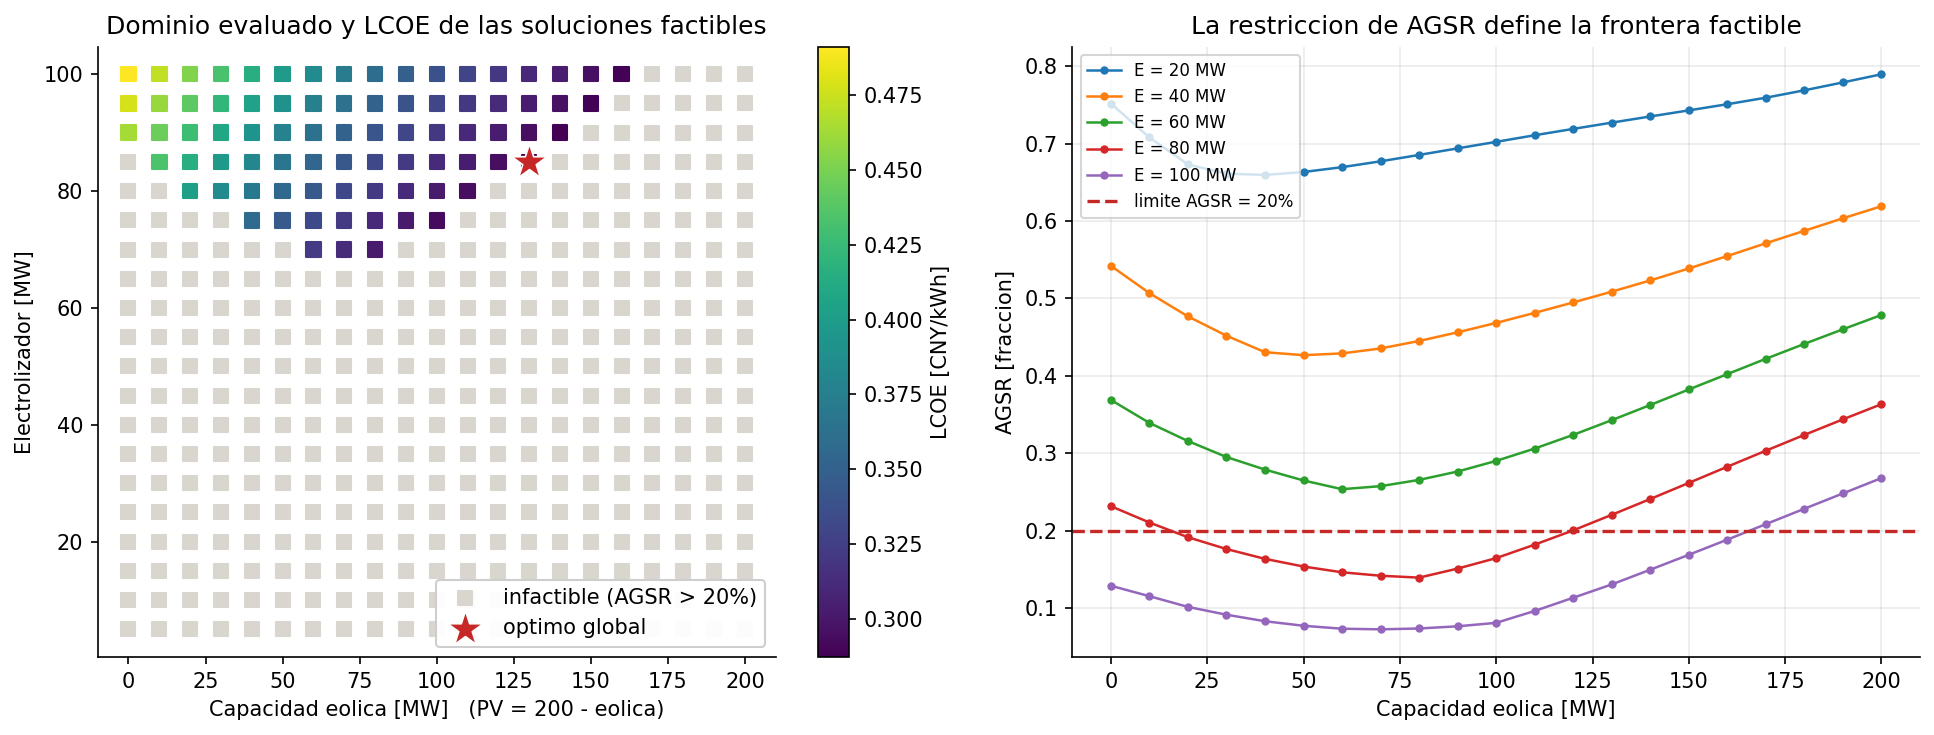
\includegraphics[width=0.95\textwidth]{figures/fig03_dominio_instancia_base.png}
\caption{LCOE y factibilidad de los 420 puntos de la instancia base de Li et al. La estrella identifica el mejor punto de esta malla, no un óptimo del dominio mixto.}
\label{fig:dominio_base}
\end{figure}

\subsection{Óptimos por fuerza bruta}

La Tabla~\ref{tab:fuerza_bruta_auto} resume la enumeración completa de cada instancia: diseños evaluados, fracción factible, óptimo exacto y tiempo de cómputo. En total se evaluaron \BruteForceDesignsTotal{} diseños anuales en \BruteForceElapsedHours{} horas de cómputo, con una diferencia relativa máxima de \MaxControlRelDiff{} entre la réplica vectorizada y el simulador oficial en las celdas de control.

\TablaFuerzaBrutaAuto

Los óptimos exactos son LCOE $=\BFALCOE$ CNY/kWh en I1 ($W=\BFAWind$ MW, $E=\BFAElectrolyzer$ MW, batería de \BFABattery{} MW durante \BFADuration{} h), \BFBLCOE{} en I2 ($W=\BFBWind$, $E=\BFBElectrolyzer$, \BFBBattery{} MW $\times$ \BFBDuration{} h), \BFCLCOE{} en I3 ($W=\BFCWind$, $E=\BFCElectrolyzer$, \BFCBattery{} MW $\times$ \BFCDuration{} h) y \BFDLCOE{} en I4 ($W=\BFDWind$, $E=\BFDElectrolyzer$, \BFDBattery{} MW $\times$ \BFDDuration{} h). En las cuatro instancias el óptimo se sitúa sobre el borde de la restricción C5, con AGSR de \BFAAGSR, \BFBAGSR, \BFCAGSR{} y \BFDAGSR{} respectivamente, y el diseño un paso de malla más allá en $W$ viola esa restricción: la fracción vendida a la red es lo que detiene la mejora, no el costo. Reducir el límite a 0,10 (I2) encarece el óptimo en más de un diez por ciento y desplaza el diseño hacia menos eólica y más electrólisis; refinar los catálogos (I3) permite un óptimo marginalmente mejor que el de I1 al disponer de combinaciones intermedias; y la escala de 300 MW (I4) reduce el LCOE por el reparto del almacenamiento de hidrógeno fijo sobre más energía.

\begin{figure}[H]
\centering
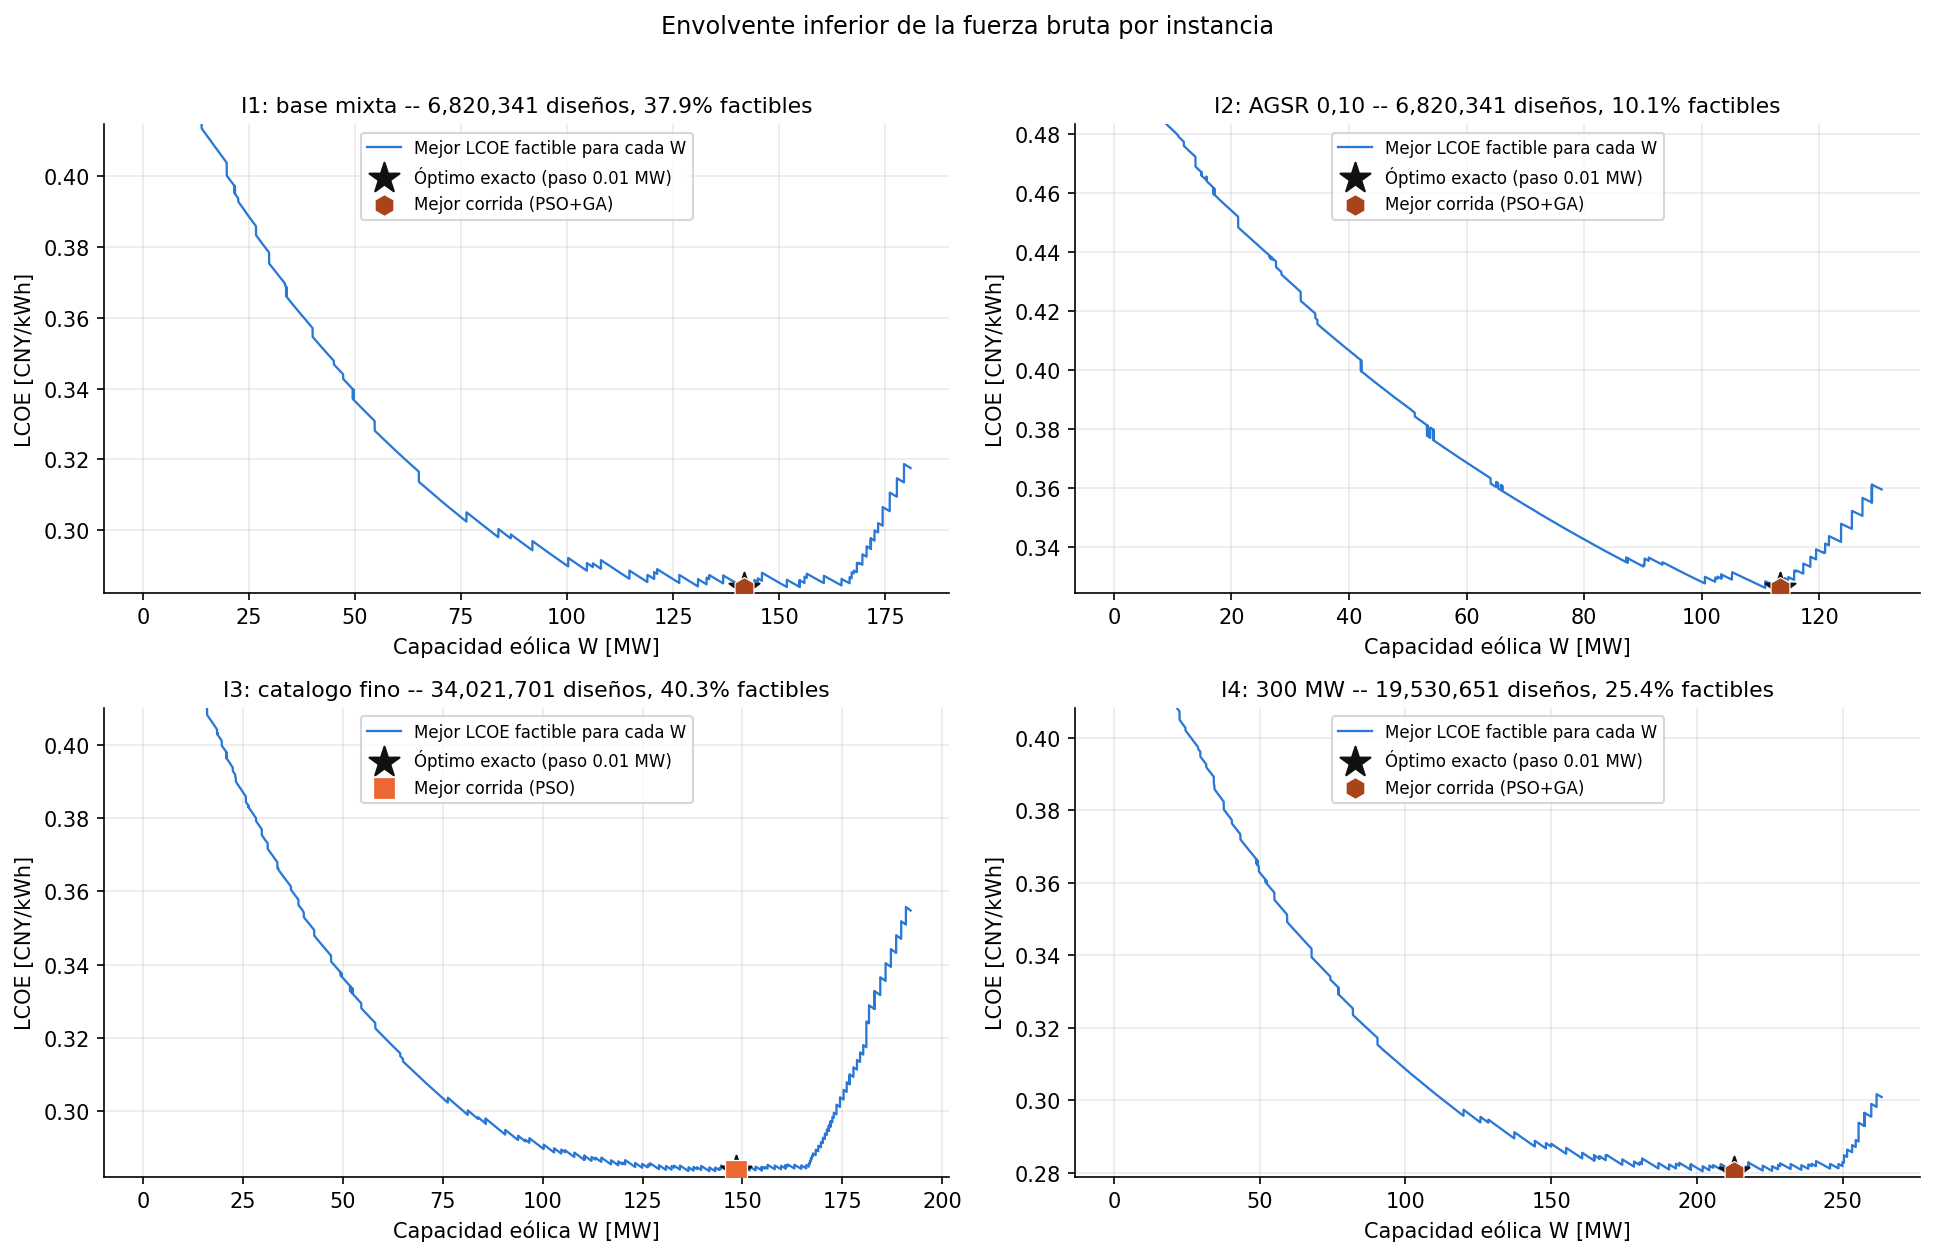
\includegraphics[width=0.98\textwidth]{figures/fig10_envolvente_fuerza_bruta.png}
\caption{Envolvente inferior de la fuerza bruta por instancia: mejor LCOE factible entre todos los catálogos para cada valor de $W$. La estrella es el óptimo exacto y el marcador coloreado la mejor corrida estocástica de la instancia.}
\label{fig:envolvente}
\end{figure}

La Figura~\ref{fig:envolvente} muestra la geometría que los algoritmos deben recorrer: la envolvente sólo existe donde hay diseños factibles, desciende suavemente hasta el óptimo y termina abruptamente en el borde de C5. La Tabla~\ref{tab:comparacion_optimo_auto} compara el óptimo exacto con la mejor corrida estocástica de cada instancia; las brechas son de \BestRunAGapPct\,\% (I1, \BestRunAAlgorithm), \BestRunBGapPct\,\% (I2, \BestRunBAlgorithm), \BestRunCGapPct\,\% (I3, \BestRunCAlgorithm) y \BestRunDGapPct\,\% (I4, \BestRunDAlgorithm). Una brecha negativa significa que el optimizador, con $W$ continuo, halló un diseño entre dos nodos de la malla de 0,01 MW.

\TablaComparacionOptimoAuto

\section{Comparación de los optimizadores por instancia}

Se ejecutaron \TotalRuns{} corridas y \TotalDesignRequests{} solicitudes de evaluación de diseños anuales. Cada una recorre 8.760 pasos horarios, por lo que el total solicitado equivale aproximadamente a \RequestedHourlySteps{} pasos; las propuestas duplicadas se contabilizan dentro del presupuesto aunque la memoria intermedia evite repetir la simulación. Las Figuras~\ref{fig:convergencia} y~\ref{fig:dispersion} muestran la convergencia y la distribución final en las cuatro instancias; las tablas siguientes detallan cada una.

\begin{figure}[H]
\centering
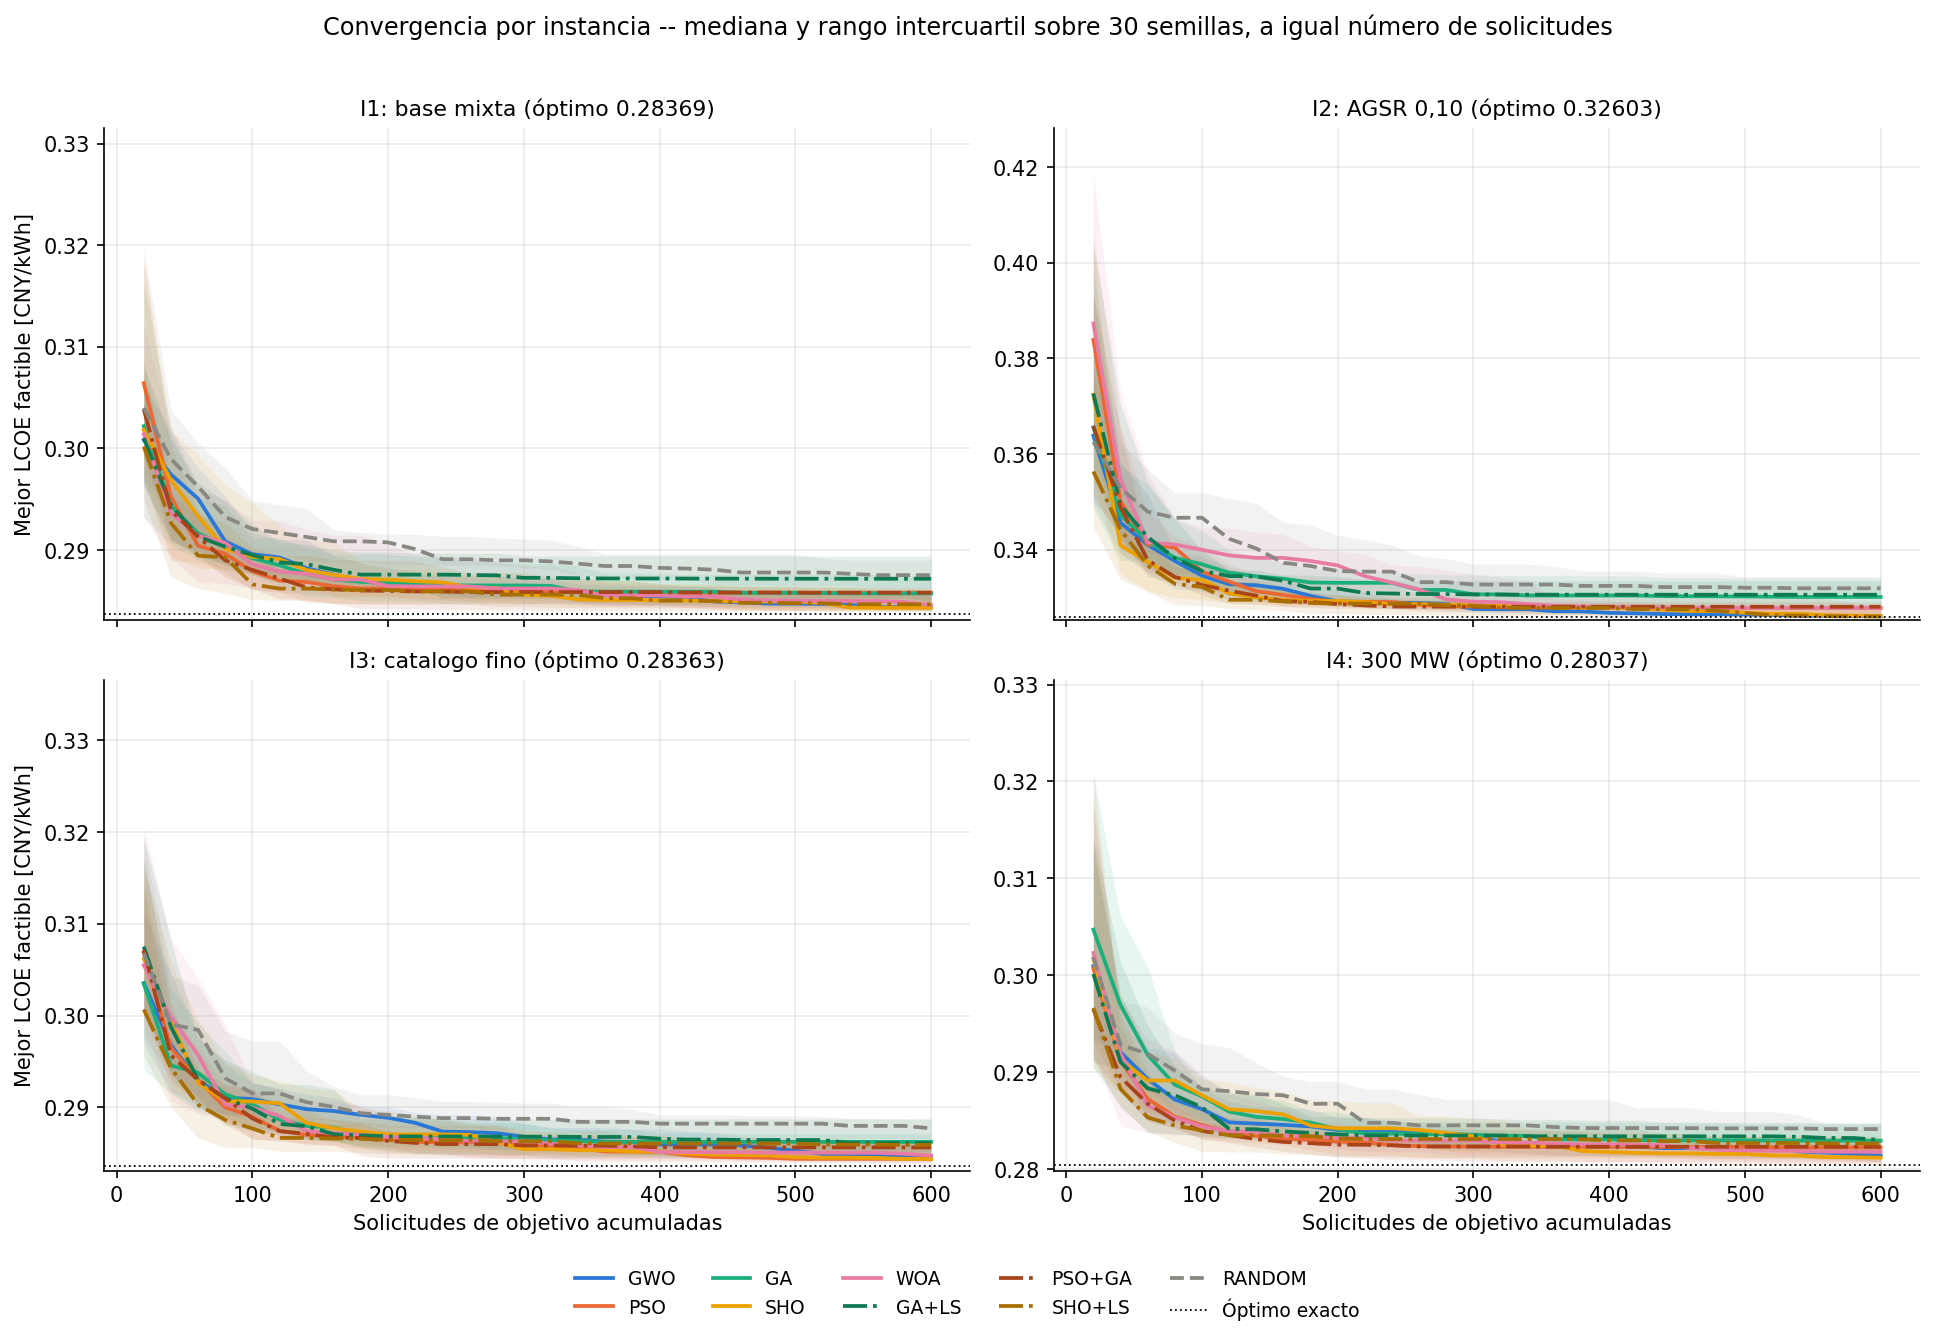
\includegraphics[width=0.98\textwidth]{figures/fig05_convergencia.png}
\caption{Mediana e intervalo intercuartílico del mejor LCOE factible a igual número de solicitudes, por instancia. La línea punteada es el óptimo exacto.}
\label{fig:convergencia}
\end{figure}

\begin{figure}[H]
\centering
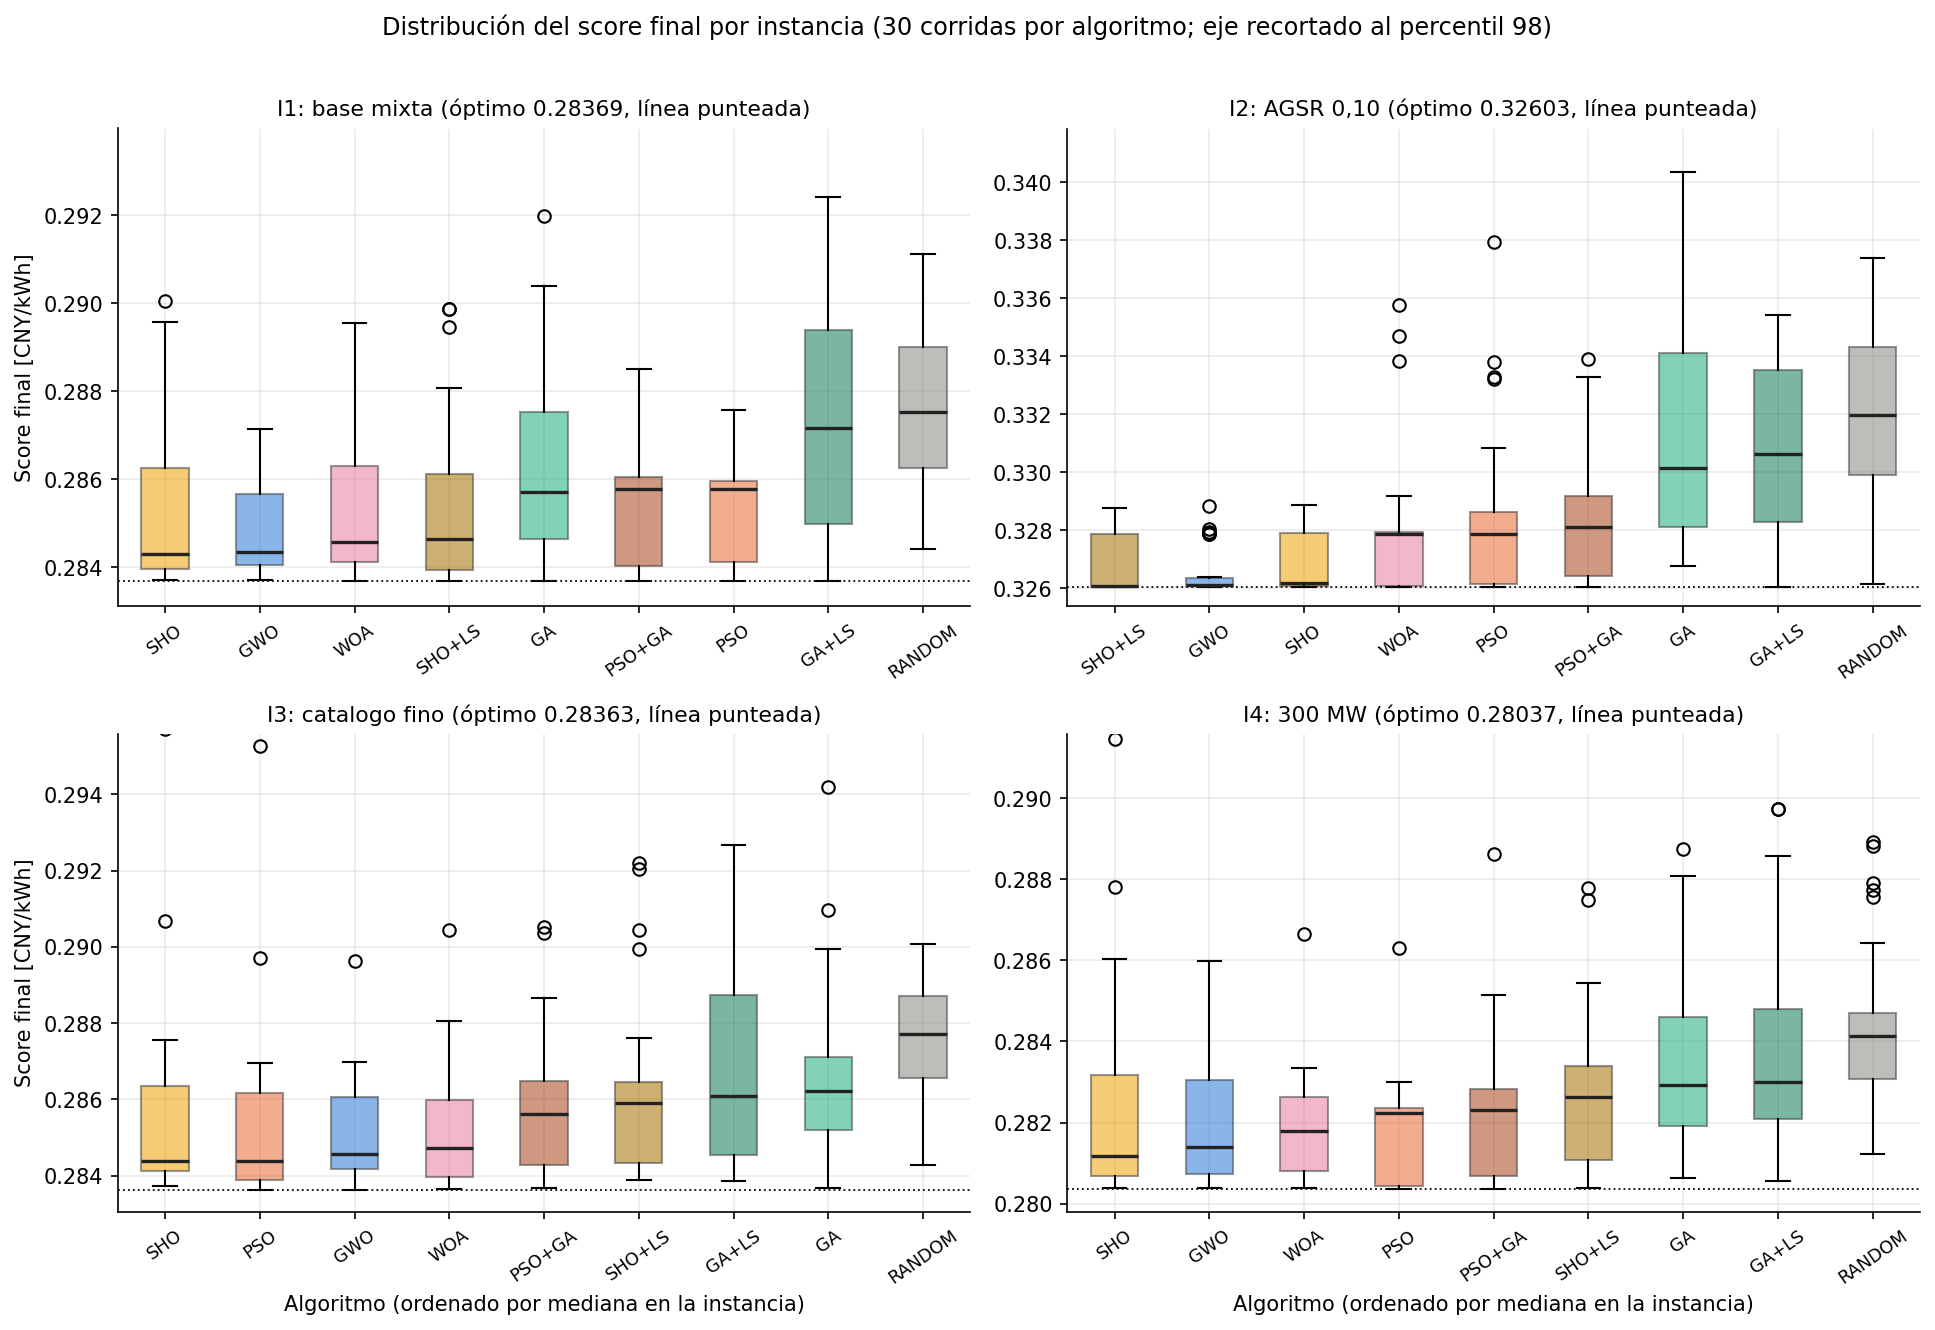
\includegraphics[width=0.98\textwidth]{figures/fig06_distribucion_scores.png}
\caption{Distribución del LCOE final de las \Replicates{} ejecuciones independientes por algoritmo e instancia, ordenadas por mediana dentro de cada instancia.}
\label{fig:dispersion}
\end{figure}

\subsection{I1: instancia mixta de referencia}

\TablaRankingAutoA
\TablaExitoAutoA
\TablaComputoAutoA
\TablaParesPlanificadosAutoA

Por mediana, \TopMedianA{} ocupa la primera posición con una brecha mediana de \TopMedianGapA\,\% respecto del óptimo exacto, seguido de \SecondMedianA; \BottomMedianA{} ocupa la última y la búsqueda aleatoria el lugar \RandomRankA{} con brecha mediana de \RandomMedianGapA\,\%. Frente a esa línea base, muestran ventaja detectable tras Holm \BetterThanRandomA; sin diferencia detectable, \NoDifferenceFromRandomA; con desventaja detectable, \WorseThanRandomA. Esta última categoría expresa ausencia de evidencia y no igualdad algorítmica. Entre los híbridos, superan la mediana de su padre \HybridsBeatParentA; los contrastes híbrido--padre significativos son \HybridsSignificantA.

\subsection{I2: región factible estrecha}

\TablaRankingAutoB
\TablaExitoAutoB
\TablaComputoAutoB
\TablaParesPlanificadosAutoB

Con el límite de ventas a red reducido a la mitad, \TopMedianB{} ocupa la primera posición (brecha mediana \TopMedianGapB\,\%), seguido de \SecondMedianB; \BottomMedianB{} ocupa la última y la búsqueda aleatoria el lugar \RandomRankB{} (brecha mediana \RandomMedianGapB\,\%). Ventaja detectable frente a la línea base: \BetterThanRandomB; sin diferencia detectable: \NoDifferenceFromRandomB; desventaja detectable: \WorseThanRandomB. Superan la mediana de su padre \HybridsBeatParentB; contrastes híbrido--padre significativos: \HybridsSignificantB. Como mínimo \FeasibleRunsMinB{} de las \Replicates{} corridas de cada algoritmo terminaron en un diseño factible.

\subsection{I3: catálogos finos}

\TablaRankingAutoC
\TablaExitoAutoC
\TablaComputoAutoC
\TablaParesPlanificadosAutoC

Con cinco veces más combinaciones discretas sobre la misma región física, \TopMedianC{} ocupa la primera posición (brecha mediana \TopMedianGapC\,\%), seguido de \SecondMedianC; \BottomMedianC{} ocupa la última y la búsqueda aleatoria el lugar \RandomRankC{} (brecha mediana \RandomMedianGapC\,\%). Ventaja detectable frente a la línea base: \BetterThanRandomC; sin diferencia detectable: \NoDifferenceFromRandomC; desventaja detectable: \WorseThanRandomC. Superan la mediana de su padre \HybridsBeatParentC; contrastes híbrido--padre significativos: \HybridsSignificantC.

\subsection{I4: escala de 300 MW}

\TablaRankingAutoD
\TablaExitoAutoD
\TablaComputoAutoD
\TablaParesPlanificadosAutoD

A escala de 300 MW, \TopMedianD{} ocupa la primera posición (brecha mediana \TopMedianGapD\,\%), seguido de \SecondMedianD; \BottomMedianD{} ocupa la última y la búsqueda aleatoria el lugar \RandomRankD{} (brecha mediana \RandomMedianGapD\,\%). Ventaja detectable frente a la línea base: \BetterThanRandomD; sin diferencia detectable: \NoDifferenceFromRandomD; desventaja detectable: \WorseThanRandomD. Superan la mediana de su padre \HybridsBeatParentD; contrastes híbrido--padre significativos: \HybridsSignificantD.

\section{Lectura transversal}

\TablaRankingTransversalAuto

El rango medio sobre las cuatro instancias sitúa en primer lugar a \BestMeanRankAlgorithm{} (rango medio \BestMeanRank) y en segundo a \SecondMeanRankAlgorithm{} (\SecondMeanRank); \WorstMeanRankAlgorithm{} ocupa el último lugar y la búsqueda aleatoria obtiene un rango medio de \RandomMeanRank. El orden es descriptivo: resume cuatro instancias paramétricas del mismo sitio y año, no una población de problemas, y las diferencias de rango entre algoritmos vecinos no son evidencia de superioridad. Las columnas de brecha y éxito medios permiten leer el mismo cuadro en términos prácticos: cuán lejos del óptimo queda una corrida típica y con qué frecuencia queda a menos de 0,5\,\% de él.

Los mecanismos de movimiento ofrecen hipótesis para interpretar las curvas: memoria personal y social en PSO, tres líderes en GWO, recombinación en GA, cambios de rama o agrupación en WOA y SHO, intensificación local en GA+LS y SHO+LS, y diversidad estructurada en PSO+GA. Sin embargo, el experimento sólo contiene ablaciones para el componente añadido por cada híbrido; en los clásicos la explicación causal por operador se mantiene como vacío metodológico, no como conclusión demostrada.

\section{Híbridos frente a sus padres}

\TablaHibridosAuto

\begin{figure}[H]
\centering
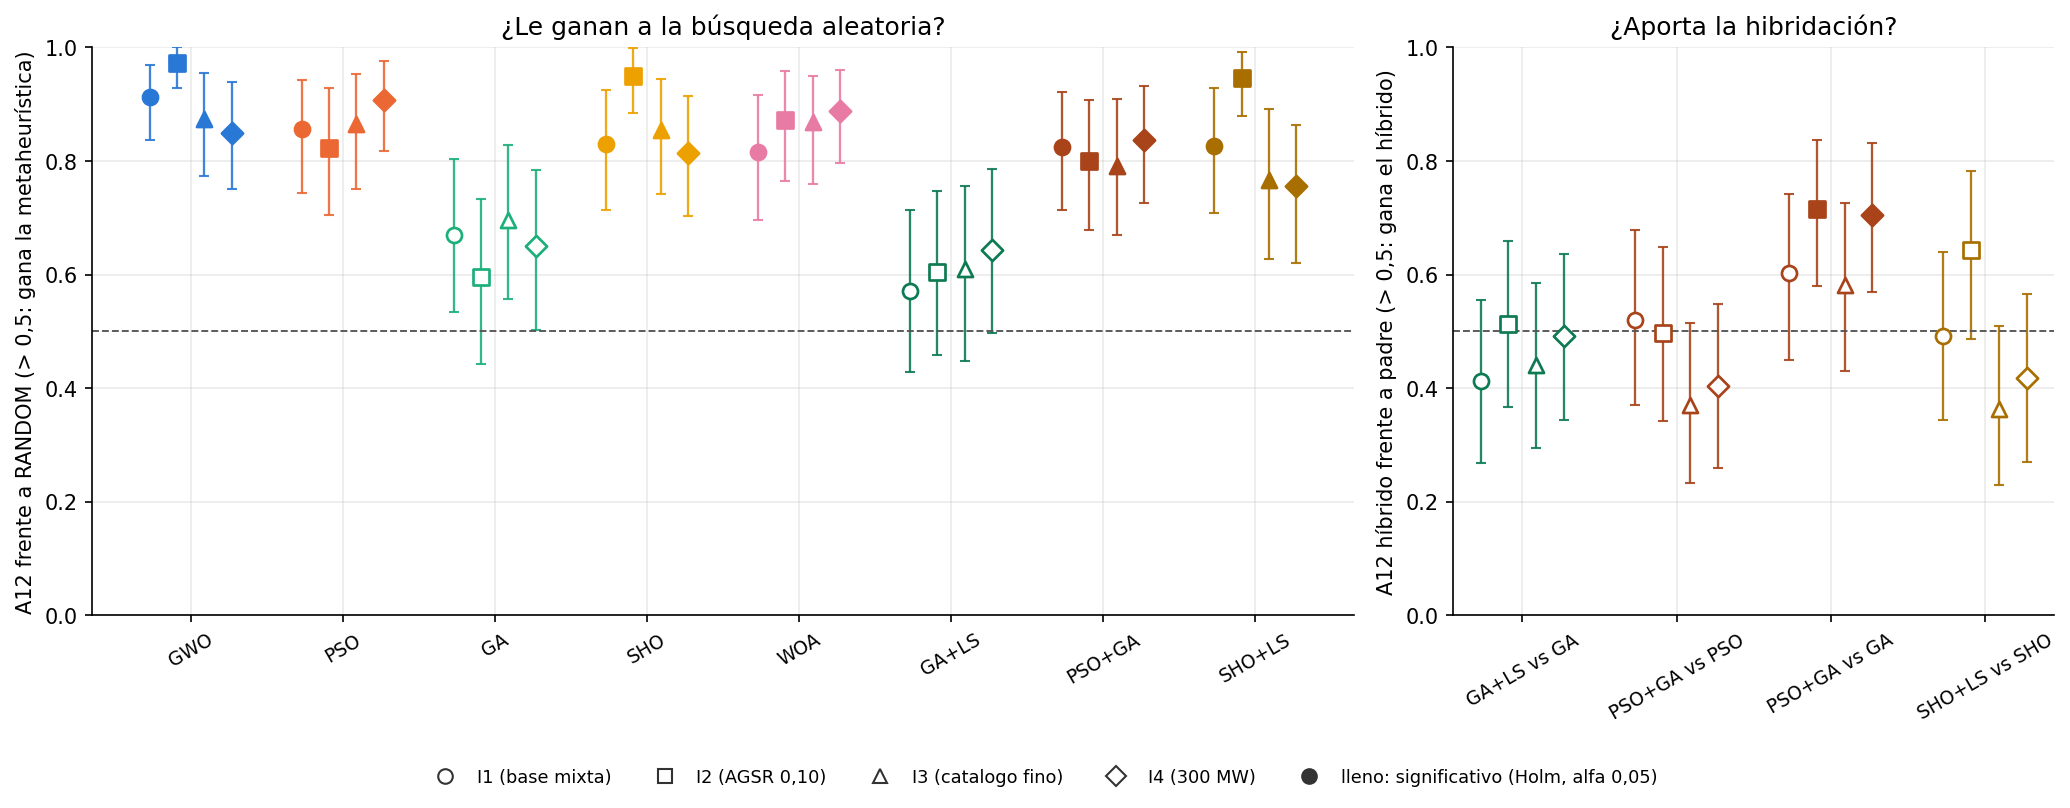
\includegraphics[width=0.98\textwidth]{figures/fig07_contrastes_planificados.png}
\caption{Contrastes planificados: $A_{12}$ con intervalo bootstrap al 95\,\% de cada metaheurística frente a RANDOM (izquierda) y de cada híbrido frente a su padre (derecha), por instancia. Marcador lleno: significativo tras Holm en la familia de la instancia.}
\label{fig:contrastes}
\end{figure}

La pregunta central de la extensión es si la hibridación aporta algo respecto del método del que parte. De los \HybridContrastsTotal{} contrastes híbrido--padre (cuatro por instancia), el híbrido obtiene mejor mediana que su padre en \HybridWinsCount{} y la diferencia es significativa tras Holm en \HybridSignificantCount{}: \HybridSignificantWins{} a favor del híbrido y \HybridSignificantLosses{} en su contra. La Tabla~\ref{tab:hibridos_auto} y la Figura~\ref{fig:contrastes} muestran que el efecto depende del par y de la instancia, lo que es coherente con el teorema de la no existencia de almuerzo gratis: añadir una búsqueda local o un operador genético redistribuye el presupuesto entre exploración y explotación, y el saldo de esa redistribución cambia con la geometría de la región factible. Las columnas de solicitudes de búsqueda local de las tablas de cómputo cuantifican cuánto presupuesto consumió la intensificación en cada instancia.

Tres patrones concretos se desprenden de la tabla. Primero, los dos contrastes significativos corresponden a PSO+GA frente a GA (I2 e I4), ambos a favor del híbrido, mientras que PSO+GA frente a PSO no se distingue en ninguna instancia ($A_{12}$ entre 0,37 y 0,52): el híbrido hereda la calidad del bucle del enjambre, y reemplazar el cuarto peor de las partículas por hijos genéticos ni mejora ni empeora al PSO puro bajo este presupuesto. Segundo, SHO+LS ocupa el primer lugar por mediana en I2, la instancia de región factible estrecha, y supera a SHO en mediana sólo allí; en I3 e I4 cae al sexto lugar. La búsqueda local consume entre 66 y 69 solicitudes por corrida, un 11\,\% del presupuesto, que en una región estrecha se invierten en afinar $W$ sobre el borde de C5 y que en un espacio discreto cinco veces mayor se restan a la exploración. Tercero, GA+LS no mejora a GA en ninguna instancia de forma detectable: parte de un método cuyo presupuesto ya se gasta en más de un 30\,\% en diseños repetidos (unas 180 a 207 solicitudes duplicadas por corrida en GA, 143 a 153 en GA+LS), y la búsqueda local añade cerca de 97 solicitudes más de intensificación sobre un individuo que el elitismo ya conserva. Las mejores corridas individuales de I1, I2 e I4 corresponden, sin embargo, a PSO+GA, y la de I3 a PSO, todas por debajo del óptimo discretizado gracias a $W$ continuo.

\section{Análisis de sensibilidad}

\TablaSensAGSRAuto
\TablaSensCargaAuto

\begin{figure}[H]
\centering
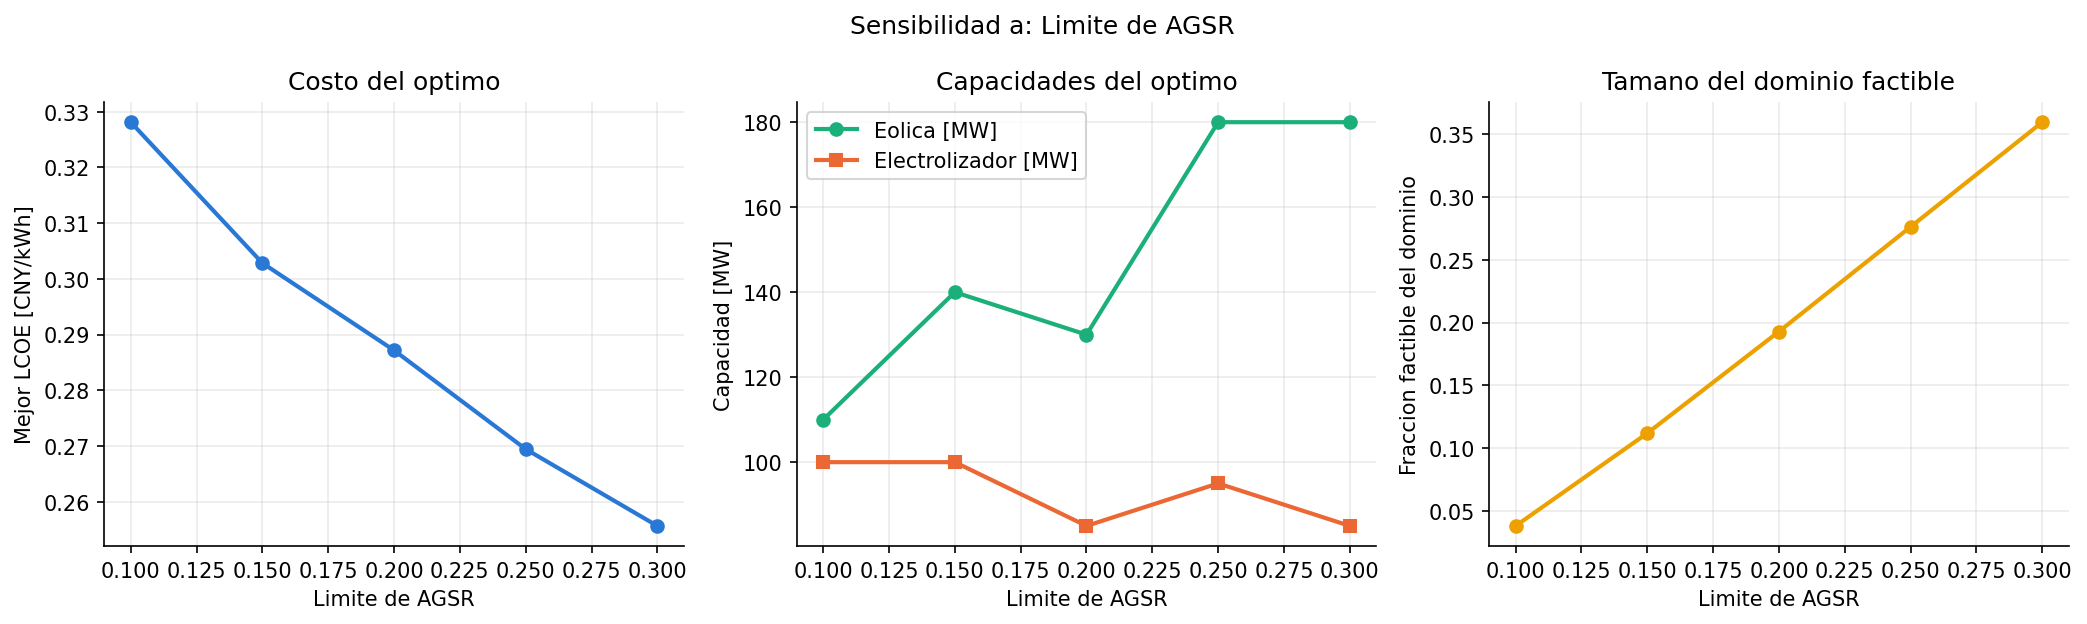
\includegraphics[width=0.96\textwidth]{figures/fig08_sensibilidad_agsr.png}
\caption{Sensibilidad determinista de la malla base al límite de fracción anual vendida a red.}
\label{fig:sens_agsr}
\end{figure}

\begin{figure}[H]
\centering
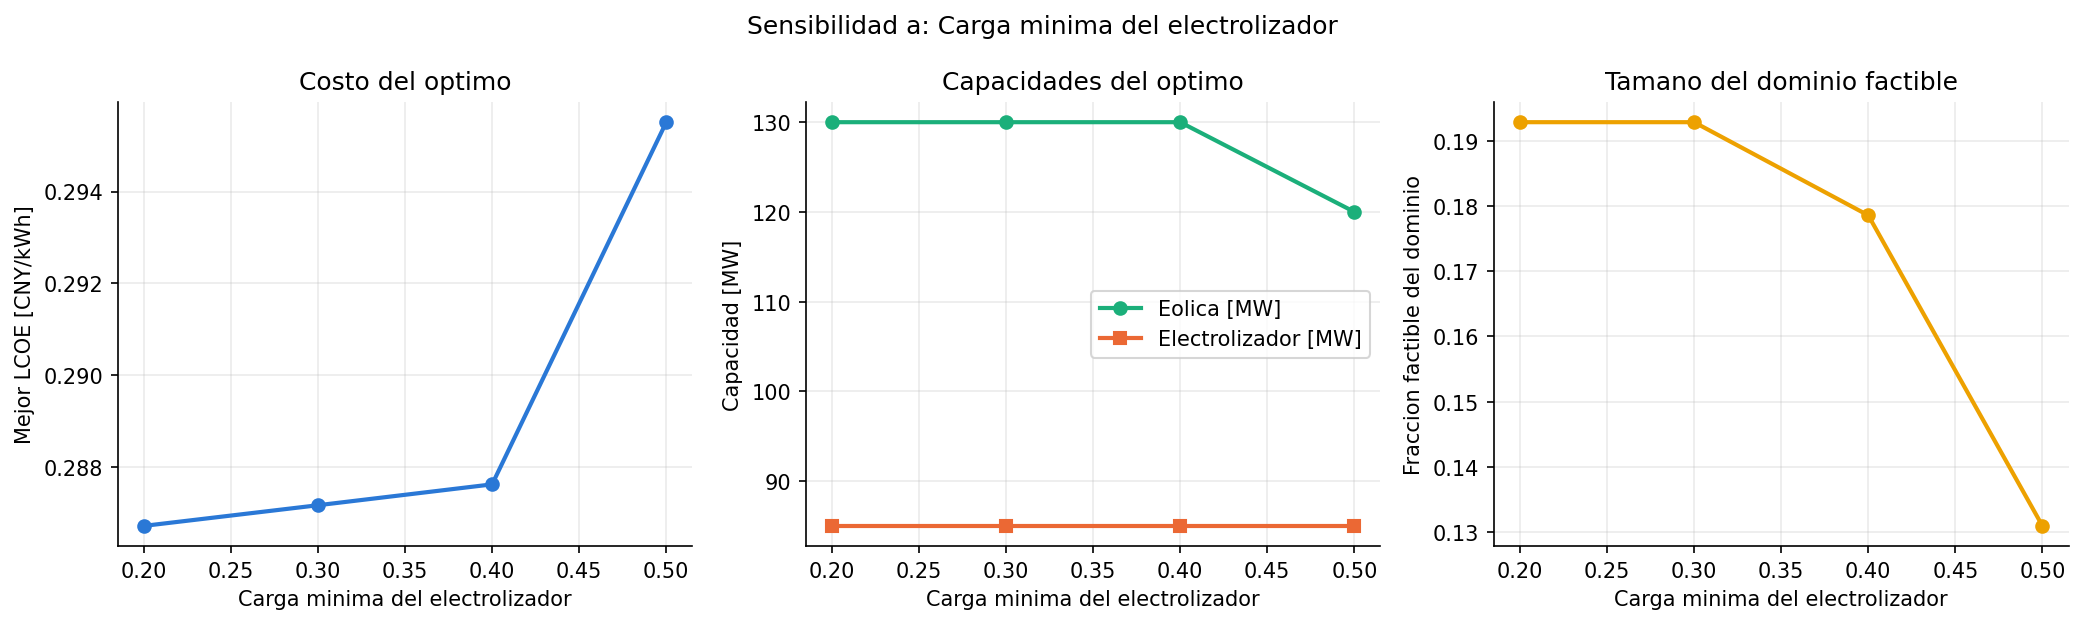
\includegraphics[width=0.96\textwidth]{figures/fig09_sensibilidad_carga_minima.png}
\caption{Sensibilidad determinista de la malla base a la carga mínima del electrolizador.}
\label{fig:sens_carga}
\end{figure}

Los barridos separan el efecto de las restricciones del ruido de los optimizadores. Muestran cómo cambian simultáneamente el tamaño de la región factible y el mejor punto de la malla base; no constituyen una prueba de robustez del ranking algorítmico. El barrido del límite de AGSR anticipa, sobre la malla base, el estrechamiento que la instancia I2 impone al dominio mixto.

\section{Verificaciones y alcance de los resultados}

Las \TotalRuns{} corridas registraron exactamente \RequestsPerRun{} solicitudes cada una y el residuo máximo de balance observado fue \texttt{\MaxBalanceResidual} MW; como mínimo \MinFeasibleRuns{} de las \Replicates{} corridas de cada algoritmo e instancia terminaron en un diseño factible. GWO, SHO, WOA y la inyección genética de PSO+GA superaron pruebas de una actualización determinista contra sus ecuaciones; la búsqueda local superó las pruebas de convergencia, presupuesto y ausencia de duplicados; los tres híbridos produjeron exactamente \Iterations{} puntos de control por corrida; y clásicos e híbridos superaron las pruebas de dirección y límites sobre Sphere y Rastrigin. La corrida de I1 reproduce bit a bit la comparativa previa de seis algoritmos.

Los resultados continúan condicionados por un solo emplazamiento aproximado y un solo año meteorológico; por instancias que varían una restricción, la finura de los catálogos y la escala, pero no el recurso ni la estructura de costos; por la ausencia de una demanda explícita de hidrógeno; por la idealización continua de $W$; por la regla declarada para operacionalizar la agrupación de SHO; y por valores de la búsqueda local y de la inyección genética fijados a priori y sin ablación por operador. El experimento compara implementaciones concretas bajo un presupuesto concreto, no familias algorítmicas en general.
